\حصہ{ہذلولی تفاعل}
ہر ایسا تفاعل \عددی{f} جس کے دائرہ کار کا وسط مبدا پر واقع ہو کو ایک جفت اور ایک طاق تفاعل کا مجموعہ لکھا جا سکتا ہے:
\begin{align*}
f(x)=\underbrace{\frac{f(x)+f(-x)}{2}}_{\text{\RL{جفت حصہ}}}+\underbrace{\frac{f(x)-f(-x)}{2}}_{\text{\RL{طاق حصہ}}}
\end{align*}
یوں قوت نمائی تفاعل \عددی{e^x} کو درج ذیل لکھا جا سکتا ہے۔
\begin{align*}
e^x=\underbrace{\frac{e^x+e^{-x}}{2}}_{\text{\RL{جفت حصہ}}}+\underbrace{\frac{e^x-e^{-x}}{2}}_{\text{\RL{طاق حصہ}}}
\end{align*} 
قوت نمائی تفاعل \عددی{e^x} کا جفت اور طاق حصہ، جنہیں  بالترتیب \عددی{x} کا ہذلولی کوسائن اور ہذلولی سائن کہتے ہیں، از خود اہمیت کے حامل ہیں۔ یہ لچکدار ٹھوس مادہ میں لہروں کی حرکت، کھمبوں کے بیچ برقی تاروں کا روپ، اور دھاتی \اصطلاح{سرد کار}\حاشیہب{heat sink} میں حرارتی کی تقسیم کو بیان کرتے ہیں۔

\جزوحصہء{تعریف اور تماثل}
ہذلولی کوسائن اور ہذلولی سائن کی تعریف جدول \حوالہ{جدول_ماورائی_چھ_بنیادی_ہذلولی_تفاعل} کی پہلی دو مساواتیں پیش کرتی ہیں۔ اس جدول میں ہذلولی ٹینجنٹ، ہذلولی کوٹینجنٹ، ہذلولی سیکنٹ، اور ہذلولی کوسیکنٹ کی تعریف بھی پیش کی گئی ہیں۔ جیسا کہ ہم دیکھیں گے، ہذلولی تفاعل ان تکونیاتی تفاعل کے ساتھ کافی  ملتے جلتے ہیں جن کے توسط سے ان کے نام رکھے گئے ہیں۔ ان کو شکل \حوالہ{شکل_ماورائی_چھ_بنیادی_ہذلولی_تفاعل} میں ترسیم کیا گیا ہے۔

\begin{table}
\caption{چھ بنیادی ہذلولی تفاعل}
\label{جدول_ماورائی_چھ_بنیادی_ہذلولی_تفاعل}
\centering
\renewcommand{\arraystretch}{2.5}
\begin{tabular}{rl}
\toprule
\عددی{x} کا ہذلولی کوسائن& \عددی{\cosh=\dfrac{e^x+e^{-x}}{2}}\\
\عددی{x} کا ہذلولی سائن & \عددی{\sinh x=\dfrac{e^x-e^{-x}}{2}}\\
\عددی{x} کا ہذلولی ٹینجنٹ&\عددی{\tanh x=\dfrac{\sinh x}{\cosh x}=\dfrac{e^x-e^{-x}}{e^x+e^{-x}}}\\
\عددی{x} کا ہذلولی کوٹینجنٹ&\عددی{\coth x=\dfrac{\cosh x}{\sinh x}=\dfrac{e^x+e^{-x}}{e^x-e^{-x}}}\\
\عددی{x} کا ہذلولی سیکنٹ&\عددی{\sech x=\dfrac{1}{\cosh x}=\dfrac{2}{e^x+e^{-x}}}\\
\عددی{x} کا ہذلولی کوسیکنٹ&\عددی{\csch x=\dfrac{1}{\sinh x}=\dfrac{2}{e^x-e^{-x}}}\\
\bottomrule
\end{tabular}
\end{table}

\begin{figure}
\centering
\begin{subfigure}{0.45\textwidth}
\centering
\begin{tikzpicture}[font=\small,declare function={f(\x)=sinh(\x);g(\x)=1/2*e^(\x);k(\x)=-1/2*e^(-\x);}]
\begin{axis}[clip=false,small,axis lines=middle,xlabel={$x$},ylabel={$y$},xlabel style={at={(current axis.right of origin)},anchor=west},ylabel style={at={(current axis.above origin)},anchor=south},enlargelimits=true]
\addplot[domain=-2:2]{f(x)}node[pos=0.75,below right]{$y=\sinh x$};
\addplot[domain=-2:2]{g(x)}node[pos=0.75,above left]{$y=\dfrac{e^x}{2}$};
\addplot[domain=-2:2]{k(x)}node[pos=0.75,below right,yshift=-2ex]{$y=-\dfrac{e^{-x}}{2}$};
\end{axis}
\end{tikzpicture}
\caption{ہذلولی سائن اور اس کے قوت نما اجزاء۔}
\end{subfigure}\hfill
\begin{subfigure}{0.45\textwidth}
\centering
\begin{tikzpicture}[font=\small,declare function={f(\x)=cosh(\x);g(\x)=1/2*e^(\x);k(\x)=1/2*e^(-\x);}]
\begin{axis}[clip=false,small,axis lines=middle,xlabel={$x$},ylabel={$y$},xlabel style={at={(current axis.right of origin)},anchor=west},ylabel style={at={(current axis.above origin)},anchor=south},enlargelimits=true]
\addplot[domain=-2:2]{f(x)}node[pos=0.85,left]{$y=\cosh x$};
\addplot[domain=-2:2]{g(x)}node[pos=0.75,below right]{$y=\dfrac{e^x}{2}$};
\addplot[domain=-2:2]{k(x)}node[pos=0.25,below left]{$y=\dfrac{e^{-x}}{2}$};
\end{axis}
\end{tikzpicture}
\caption{ہذلولی کوسائن اور اس کے قوت نما اجزاء۔}
\end{subfigure}
\begin{subfigure}{0.45\textwidth}
\centering
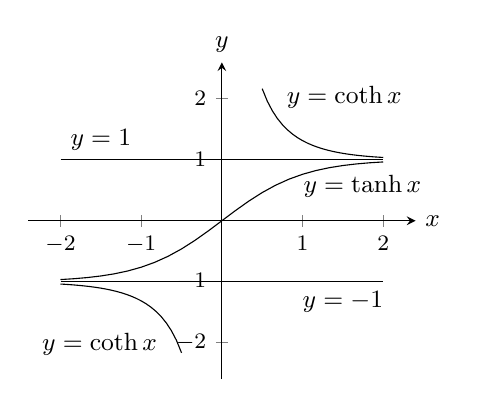
\begin{tikzpicture}[font=\small,declare function={f(\x)=tanh(\x);g(\x)=1/tanh(\x);}]
\begin{axis}[clip=false,small,axis lines=middle,xlabel={$x$},ylabel={$y$},xlabel style={at={(current axis.right of origin)},anchor=west},ylabel style={at={(current axis.above origin)},anchor=south},enlargelimits=true]
\addplot[domain=-2:2]{f(x)}node[pos=0.75,below right,yshift=1ex]{$y=\tanh x$};
\addplot[domain=0.5:2]{g(x)}node[pos=0.25,above right]{$y=\coth x$};
\addplot[domain=-0.5:-2]{g(x)}node[pos=0.25,below left]{$y=\coth x$};
\draw(-2,1)--(2,1)  (-2,-1)--(2,-1);
\draw(-1.5,1)node[above]{$y=1$}  (1.5,-1)node[below]{$y=-1$};
\end{axis}
\end{tikzpicture}
\caption{ہذلولی ٹینجنٹ اور ہذلولی کوٹینجنٹ۔}
\end{subfigure}\hfill
\begin{subfigure}{0.45\textwidth}
\centering
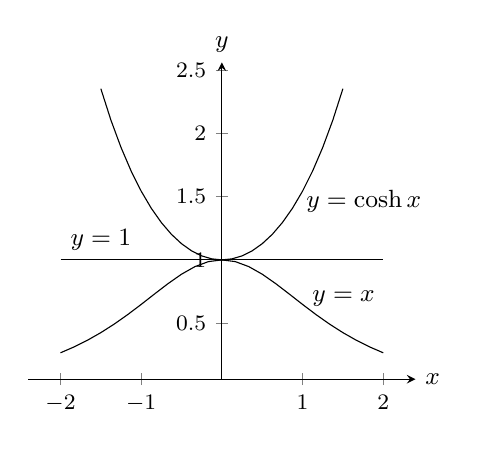
\begin{tikzpicture}[font=\small,declare function={f(\x)=cosh(\x);g(\x)=1/cosh(\x);}]
\begin{axis}[clip=false,small,axis lines=middle,xlabel={$x$},ylabel={$y$},xlabel style={at={(current axis.right of origin)},anchor=west},ylabel style={at={(current axis.above origin)},anchor=south},enlargelimits=true]
\addplot[domain=-1.5:1.5]{f(x)}node[pos=0.75,right]{$y=\cosh x$};
\addplot[domain=-2:2]{g(x)}node[pos=0.75,above right,yshift=-1ex]{$y=\sech x$};
\draw(-2,1)--(2,1);
\draw(-1.5,1)node[above]{$y=1$};
\end{axis}
\end{tikzpicture}
\caption{ہذلولی کوسائن اور ہذلولی سیکنٹ۔}
\end{subfigure}
\begin{subfigure}{0.45\textwidth}
\centering
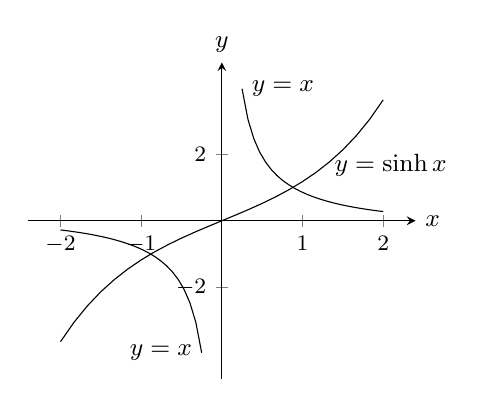
\begin{tikzpicture}[font=\small,declare function={f(\x)=sinh(\x);g(\x)=1/sinh(\x);}]
\begin{axis}[clip=false,small,axis lines=middle,xlabel={$x$},ylabel={$y$},xlabel style={at={(current axis.right of origin)},anchor=west},ylabel style={at={(current axis.above origin)},anchor=south},enlargelimits=true,ytick={-2,2}]
\addplot[domain=-2:2]{f(x)}node[pos=0.75,right]{$y=\sinh x$};
\addplot[domain=0.25:2]{g(x)}node[pos=0,right]{$y=\csch x$};
\addplot[domain=-0.25:-2]{g(x)}node[pos=0,left]{$y=\csch x$};
\end{axis}
\end{tikzpicture}
\caption{ہذلولی سائن اور ہذلولی کوسیکنٹ۔}
\end{subfigure}
\caption{چھ بنیادی ہذلولی تفاعل۔}
\label{شکل_ماورائی_چھ_بنیادی_ہذلولی_تفاعل}
\end{figure}

\جزوحصہء{تماثل}
ہذلولی تفاعل جدول \حوالہ{جدول_ماورائی_تماثل} میں دی گئی تماثل کو مطمئن کرتے ہیں۔ ماسوائے علامت، ہم ان تماثل کو تکونیاتی تفاعل سے جانتے ہیں۔

\begin{table}
\caption{ہذلولی تفاعل کے تماثل۔}
\label{جدول_ماورائی_تماثل}
\centering
\renewcommand{\arraystretch}{2}
\begin{tabular}{L}
\toprule
\sinh2x=2\sinh x \cosh x\\
\cosh2x=\cosh^2x+\sinh^2x\\
\cosh^2x=\dfrac{\cosh 2x+1}{2}\\
\sinh^2x=\dfrac{\cosh 2x-1}{2}\\
\cosh^2x-\sinh^2=1\\
\tanh^2x=1-\sech^2x\\
\coth^2x=1+\csch^2x\\
\bottomrule
\end{tabular}
\end{table} 

\جزوحصہء{تفرق اور تکمل}
چھ بنیادی ہذلولی تفاعل، قابل تفرق تفاعل \عددی{e^x} اور \عددی{e^{-x}} کے ناطق مجموعے ہیں، لہٰذا یہ ہر اس نقطہ پر قابل تفرق ہوں گے  جس پر یہ معین ہوں۔ یہاں بھی تکونیاتی تفاعل کے ساتھ مشابہت نظر آتی ہے۔ جدول \حوالہ{جدول_ماورائی_ہذلولی_کلیات_تفرق_تکمل}-ا کے کلیات تفرق سے جدول \حوالہ{جدول_ماورائی_ہذلولی_کلیات_تفرق_تکمل}-ب کے کلیات تکمل حاصل ہوتے ہیں۔ تکونیاتی تفاعل کی طرح ہذلولی تفاعل کی قیمتوں  کو بھی کیلکولیٹر سے حاصل کیا جا سکتا ہے۔

\begin{table}
\caption{ہذلولی تفاعل کے کلیات تفرق اور کلیات تکمل۔}
\label{جدول_ماورائی_ہذلولی_کلیات_تفرق_تکمل}
\centering
\renewcommand{\arraystretch}{2}
\begin{subtable}{0.45\textwidth}
\caption{ہذلولی تفاعل کے تفرق۔}
\centering
\begin{tabular}{L}
\toprule
\frac{\dif}{\dif x}(\sinh u)=\cosh u\frac{\dif u}{\dif x}\\
\frac{\dif}{\dif x}(\cosh u)=\sinh u\frac{\dif u}{\dif x}\\
\frac{\dif}{\dif x}(\tanh u)=\sech^2 u\frac{\dif u}{\dif x}\\
\frac{\dif}{\dif x}(\coth u)=-\csch^2 u\frac{\dif u}{\dif x}\\
\frac{\dif}{\dif x}(\sech u)=-\sech u\tanh u \frac{\dif u}{\dif x}\\
\frac{\dif}{\dif x}(\csch u)=-\csch u\coth u\frac{\dif u}{\dif x}\\
\bottomrule
\end{tabular}
\end{subtable}\hfill
\begin{subtable}{0.45\textwidth}
\caption{ہذلولی تفاعل کے تکمل۔}
\centering
\begin{tabular}{L}
\toprule
\frac{\dif}{\dif x}(\sinh u)=\cosh u\frac{\dif u}{\dif x}\\
\frac{\dif}{\dif x}(\cosh u)=\sinh u\frac{\dif u}{\dif x}\\
\frac{\dif}{\dif x}(\tanh u)=\sech^2 u\frac{\dif u}{\dif x}\\
\frac{\dif}{\dif x}(\coth u)=-\csch^2 u\frac{\dif u}{\dif x}\\
\frac{\dif}{\dif x}(\sech u)=-\sech u\tanh u \frac{\dif u}{\dif x}\\
\frac{\dif}{\dif x}(\csch u)=-\csch u\coth u\frac{\dif u}{\dif x}\\
\bottomrule
\end{tabular}
\end{subtable}
\end{table} 

\ابتدا{مثال}
\begin{align*}
\frac{\dif}{\dif t}(\tanh\sqrt{1+t^2})&=\sech^2\sqrt{1+t^2}\cdot\frac{\dif}{\dif t}(\sqrt{1+t^2})\\
&=\frac{t}{\sqrt{1+t^2}}\sech^2\sqrt{1+t^2}
\end{align*}
\انتہا{مثال}
%=========================
\ابتدا{مثال}
\begin{align*}
\int\coth 5x\dif x&=\int\frac{\cosh 5x}{\sinh 5x}\dif x=\frac{1}{5}\int\frac{\dif u}{u}&&u=\sinh 5x\\
&=\frac{1}{5}\ln\abs{u}+C=\frac{1}{5}\ln\abs{\sinh 5x}+C
\end{align*}
\انتہا{مثال}
%======================
\ابتدا{مثال}
\begin{align*}
\int_0^1\sinh^2x\dif x&=\int_0^1\frac{\cosh 2x-1}{2}\dif x&&\text{\RL{جدول \حوالہ{جدول_ماورائی_تماثل}}}\\
&=\frac{1}{2}\int_0^1(\cosh 2x-1)\dif x=\frac{1}{2}\left[\frac{\sinh 2x}{2}-x\right]_0^1\\
&=\frac{\sinh 2}{4}-\frac{1}{2}\approx \num{0.40672}
\end{align*}
\انتہا{مثال}
%==========================
\ابتدا{مثال}
\begin{align*}
\int_0^{\ln 2}4e^x\sinh x\dif x&=\int_0^{\ln 2}4e^x\frac{e^x-e^{-x}}{2}\dif x=\int_0^{\ln 2}(2e^{2x}-2)\dif x\\
&=\left[e^{2x}-2x\right]_0^{\ln 2}=(e^{2\ln 2}-2\ln 2)-(1-0)\\
&=4-2\ln 2-1\\
&\approx \num{1.6137}
\end{align*}
\انتہا{مثال}
%========================

\جزوحصہء{الٹ ہذلولی تفاعل}
ہم چھ بنیادی ہذلولی تفاعل کو تکمل میں استعمال کرتے ہیں۔ چونکہ \عددی{\tfrac{\dif}{\dif x}(\sinh x)=\cosh x>0} لہٰذا \عددی{x} کے لحاظ سے ہذلولی سائن بڑھتا تفاعل ہے۔ ہم اس کے الٹ کو درج ذیل سے ظاہر کرتے ہیں۔
\begin{align*}
y=\sinh^{-1}x
\end{align*}
وقفہ \عددی{-\infty<x<\infty} میں ہر \عددی{x} کے لئے \عددی{y=\sinh^{-1}x} کی قیمت وہ ہو گی جس کے ہذلولی سائن  کی قیمت \عددی{x} ہو۔ تفاعل \عددی{y=\sinh x} اور \عددی{y=\sinh^{-1}x} کے ترسیمات کو شکل \حوالہ{شکل_ماورائی_چھ_بنیادی_الٹ_ہذلولی_ترسیمات}-ا میں پیش کیا گیا ہے۔

جیسا آپ شکل \حوالہ{شکل_ماورائی_چھ_بنیادی_ہذلولی_تفاعل}-ب میں دیکھ سکتے ہیں، تفاعل \عددی{y=\cosh x} ایک ایک نہیں ہے۔ البتہ اس کی پابند شدہ روپ \عددی{y=\cosh x,\,x\ge 0} ایک ایک ہے لہٰذا اس کا الٹ پایا جائے گا جس کو درج ذیل سے ظاہر کیا جاتا ہے۔
\begin{align*}
y=\cosh^{-1}x
\end{align*}
متغیر \عددی{x\ge 1} کے ہر قیمت کے لئے وقفہ \عددی{0\le y\le\infty} میں \عددی{y=\cosh^{-1}x} ایک ایسا عدد ہو گا جس کے ہذلولی کوسائن  کی قیمت \عددی{x} ہو گی۔   تفاعل \عددی{y=\cosh x,\, x\ge 0} اور \عددی{y=\cosh^{-1}x} کی ترسیمات کو شکل \حوالہ{شکل_ماورائی_چھ_بنیادی_الٹ_ہذلولی_ترسیمات}-ب میں دکھایا گیا ہے۔
\begin{figure}
\centering
\begin{subfigure}{0.45\textwidth}
\centering
\begin{tikzpicture}[font=\scriptsize,declare function={f(\x)=sinh(\x);g(\x)=\x;}]
\begin{axis}[clip=false,small,axis lines=middle,xlabel={$x$},ylabel={$y$},xlabel style={at={(current axis.right of origin)},anchor=west},ylabel style={at={(current axis.above origin)},anchor=south},enlargelimits=true]
\addplot[domain=-1.75:1.75]{f(x)}node[above,xshift=-1ex]{$y=\sinh x$};
\addplot[domain=-2:2]({f(x)},x)node[below,xshift=1ex]{$\begin{aligned}y&=\sinh^{-1} x \\ (x&=\sinh y) \end{aligned}$};
\addplot[domain=-3:3]{g(x)}node[right]{$y=x$};
\end{axis}
\end{tikzpicture}
\caption{ہذلولی سائن اور الٹ ہذلولی سائن کے ترسیمات۔ یہ دونوں لکیر \عددی{y=x} کے لحاظ سے تشاکلی ہیں۔}
\end{subfigure}\hfill
\begin{subfigure}{0.45\textwidth}
\centering
\begin{tikzpicture}[font=\scriptsize,declare function={f(\x)=cosh(\x);g(\x)=\x;}]
\begin{axis}[clip=false,small,axis lines=middle,xlabel={$x$},ylabel={$y$},xlabel style={at={(current axis.right of origin)},anchor=west},ylabel style={at={(current axis.above origin)},anchor=south},enlargelimits=true]
\addplot[domain=0:2]{f(x)}node[above,xshift=-1ex]{$\begin{aligned}y&=\cosh x\\ x&\ge 0  \end{aligned}$};
\addplot[domain=0:2]({f(x)},x)node[below,xshift=1ex]{$\begin{aligned}y&=\cosh^{-1} x \\ (x&=\cosh y,\, y\ge 0) \end{aligned}$};
\addplot[domain=0:3]{g(x)}node[right]{$y=x$};
\end{axis}
\end{tikzpicture}
\caption{ہذلولی کوسائن اور الٹ ہذلولی کوسائن کے ترسیمات۔ یہ دونوں لکیر \عددی{y=x} کے لحاظ سے تشاکلی ہیں۔}
\end{subfigure}\hfill
\begin{subfigure}{0.45\textwidth}
\centering
\begin{tikzpicture}[font=\scriptsize,declare function={f(\x)=1/cosh(\x);g(\x)=\x;}]
\begin{axis}[clip=false,small,axis lines=middle,xlabel={$x$},ylabel={$y$},xlabel style={at={(current axis.right of origin)},anchor=west},ylabel style={at={(current axis.above origin)},anchor=south},enlargelimits=true,xtick={1,2},ytick={1,2}]
\addplot[domain=0:3]{f(x)}node[above,xshift=-1ex]{$y=\sech x\,\, x\ge 0 $};
\addplot[domain=0:3]({f(x)},x)node[right]{$\begin{aligned}y&=\sech^{-1} x \\ (x&=\sech y,\, y\ge 0) \end{aligned}$};
\addplot[domain=0:3]{g(x)}node[right]{$y=x$};
\end{axis}
\end{tikzpicture}
\caption{ہذلولی سیکنٹ اور الٹ ہذلولی سیکنٹ کے ترسیمات۔ یہ دونوں لکیر \عددی{y=x} کے لحاظ سے تشاکلی ہیں۔}
\end{subfigure}\hfill
\begin{subfigure}{0.45\textwidth}
\centering
\begin{tikzpicture}[font=\scriptsize,declare function={f(\x)=1/sinh(\x);g(\x)=\x;}]
\begin{axis}[clip=false,small,axis lines=middle,xlabel={$x$},ylabel={$y$},xlabel style={at={(current axis.right of origin)},anchor=west},ylabel style={at={(current axis.above origin)},anchor=south},enlargelimits=true,xtick={\empty},ytick={\empty}]
\addplot[domain=0.5:3]{f(x)};
\addplot[domain=-0.5:-3]{f(x)};
\draw(-1,1)node[left]{$\begin{aligned}y&=\csch^{-1}x\\ x&=\csch y   \end{aligned} $};
\end{axis}
\end{tikzpicture}
\caption{الٹ ہذلولی کوسیکنٹ کا ترسیم۔}
\end{subfigure}\hfill
\begin{subfigure}{0.45\textwidth}
\centering
\begin{tikzpicture}[font=\scriptsize,declare function={f(\x)=tanh(\x);}]
\begin{axis}[clip=false,small,axis lines=middle,xlabel={$x$},ylabel={$y$},xlabel style={at={(current axis.right of origin)},anchor=west},ylabel style={at={(current axis.above origin)},anchor=south},enlargelimits=true,xtick={-1,1},xticklabels={$\llap -1\phantom{x}$,{\rlap 1}},ytick={\empty}]
\addplot[domain=-2:2]({f(x)},x);
\draw(-1,1)node[right]{$\begin{aligned}y&=\tanh^{-1}x\\ x&=\tanh y   \end{aligned} $};
\draw(-1,-2)--(-1,2)  (1,-2)--(1,2);
\end{axis}
\end{tikzpicture}
\caption{الٹ ہذلولی ٹینجنٹ کا ترسیم۔}
\end{subfigure}\hfill
\begin{subfigure}{0.45\textwidth}
\centering
\begin{tikzpicture}[font=\scriptsize,declare function={f(\x)=1/tanh(\x);}]
\begin{axis}[clip=false,small,axis lines=middle,xlabel={$x$},ylabel={$y$},xlabel style={at={(current axis.right of origin)},anchor=west},ylabel style={at={(current axis.above origin)},anchor=south},enlargelimits=true,xtick={-1,1},xticklabels={$\llap -1\phantom{x}$,$\rlap 1$},ytick={\empty}]
\addplot[domain=0.5:2]({f(x)},x);
\addplot[domain=-0.5:-2]({f(x)},x);
\draw(-1,1)node[left]{$\begin{aligned}y&=\coth^{-1}x\\ x&=\coth y   \end{aligned} $};
\draw(-1,-2)--(-1,2)  (1,-2)--(1,2);
\end{axis}
\end{tikzpicture}
\caption{الٹ ہذلولی کوٹینجنٹ کا ترسیم۔}
\end{subfigure}
\caption{چھ بنیادی ہذلولی تفاعل کے الٹ۔}
\label{شکل_ماورائی_چھ_بنیادی_الٹ_ہذلولی_ترسیمات}
\end{figure}

تفاعل \عددی{y=\cosh x} کی طرح \عددی{y=\sech x=\tfrac{1}{\cosh x}} بھی ایک ایک نہیں ہے، البتہ \عددی{x} کو غیر منفی قیمتوں پر پابند کرنے سے  \عددی{y=\sech x} ایک ایک ہوتا ہے جس کا الٹ پایا جائے گا۔ اس الٹ کو
\begin{align*}
y=\sech^{-1}x
\end{align*}
سے ظاہر کیا جاتا ہے۔ وقفہ \عددی{(0,1]} میں \عددی{x} کی ہر قیمت کے لئے \عددی{y=\sech^{-1}x} وہ عدد ہو گا جس کا الٹ ہذلولی سیکنٹ \عددی{x} ہو گا۔

ہذلولی کوسیکنٹ، ہذلولی ٹینجنٹ اور ہذلولی کوٹینجنٹ اپنے اپنے دائرہ کار پر  ایک ایک ہیں لہٰذا ان کے الٹ پائے جائیں گے جنہیں
\begin{align*}
y=\csch^{-1}x,\quad y=\tanh^{-1}x,\quad y=\coth^{-1}x
\end{align*}
سے ظاہر کیا گیا ہے کو شکل \حوالہ{شکل_ماورائی_چھ_بنیادی_الٹ_ہذلولی_ترسیمات}-د، ہ، و میں ترسیم کیا گیا ہے۔

\جزوحصہء{کارآمد تماثل}
چند کارآمد تماثل کو جدول \حوالہ{جدول_ماورائی_چند_کارآمد_تماثل} میں پیش کیا گیا ہے۔ تفاعل \عددی{\cosh^{-1}x}، \عددی{\sinh^{-1}x} اور \عددی{\tanh^{-1}x} کی قیمتیں جانتے ہوئے ان تماثل کی استعمال سے  \عددی{\sech^{-1}x}، \عددی{\csch^{-1}x} اور \عددی{\coth^{-1}x} کی قیمتیں حاصل کی جا سکتی ہیں۔

\begin{table}
\caption{الٹ ہذلولی تفاعل کے چند کار آمد تماثل}
\label{جدول_ماورائی_چند_کارآمد_تماثل}
\centering
\renewcommand{\arraystretch}{2}
\begin{tabular}{L}
\toprule
\sech^{-1}x=\cosh^{-1}\frac{1}{x}\\
\csch^{-1}x=\sinh^{-1}\frac{1}{x}\\
\coth^{-1}x=\tanh^{-1}\frac{1}{x}\\
\bottomrule
\end{tabular}
\end{table}

\جزوحصہء{الٹ ہذلولی تفاعل کے تفرق اور تکمل}
الٹ ہذلولی تفاعل کا اہم ترین استعمال،  تکمل کے ذریعہ  جدول \حوالہ{جدول_ماورائی_الٹ_ہذلولی_تفرق} میں کلیات تفرق سے کلیات تکمل کا حصول ہے۔

تفاعل \عددی{\tanh^{-1}u} اور \عددی{\coth^{-1}u} کے تفرق پر \عددی{\abs{u}<a} اور \عددی{\abs{u}>1} کی پابندی، ان تفاعل پر پابندی کی بنا ہے (شکل \حوالہ{شکل_ماورائی_چھ_بنیادی_الٹ_ہذلولی_ترسیمات}-ہ، و دیکھیں)۔ کلیات تفرق کو کلیات تکمل میں تبدیل کرتے وقت \عددی{\abs{u}<1} اور \عددی{\abs{u}>1} میں امتیاز اہمیت حاصل کرتا ہے۔ اگر \عددی{\abs{u}<1} ہو تب \عددی{\tfrac{1}{1-u^2}} کا تکمل \عددی{\tanh^{-1}u+C} ہو گا۔ اس کے برعکس \عددی{\abs{u}>1} کی صورت میں تکمل \عددی{\coth^{-1}u+C} ہو گا۔

\begin{table}
\caption{الٹ ہذلولی تفاعل کے تفرق۔}
\label{جدول_ماورائی_الٹ_ہذلولی_تفرق}
\centering
\renewcommand{\arraystretch}{2}
\begin{tabular}{L}
\toprule
\frac{\dif\,(\sinh^{-1}u)}{\dif x}=\frac{1}{\sqrt{1+u^2}}\frac{\dif u}{\dif x}\\
\frac{\dif\,(\cosh^{-1}u)}{\dif x}=\frac{1}{\sqrt{u^2-1}}\frac{\dif u}{\dif x},\quad u>1\\
\frac{\dif\,(\tanh^{-1}u)}{\dif x}=\frac{1}{1-u^2}\frac{\dif u}{\dif x},\quad \abs{u}<1\\
\frac{\dif\,(\coth^{-1}u)}{\dif x}=\frac{1}{1-u^2}\frac{\dif u}{\dif x},\quad \abs{u}>1\\
\frac{\dif\,(\sech^{-1}u)}{\dif x}=\frac{-1}{u\sqrt{1-u^2}}\frac{\dif u}{\dif x},\quad 0<u<1\\
\frac{\dif\,(\csch^{-1}u)}{\dif x}=\frac{-1}{\abs{u}\sqrt{1+u^2}}\frac{\dif u}{\dif x},\quad u\ne 0\\
\bottomrule
\end{tabular}
\end{table}

\ابتدا{مثال}
دکھائیں کہ اگر متغیر \عددی{x} کا \عددی{u} قابل تفرق تفاعل ہو اور جس کی قیمتیں \عددی{1} سے زیادہ ہوں تب درج ذیل ہو گا۔
\begin{align*}
\frac{\dif}{\dif x}(\cosh^{-1}u)=\frac{1}{\sqrt{u^2-1}}\frac{\dif u}{\dif x}
\end{align*}
حل:\quad
ہم پہلے عددی{x>1} کی صورت میں \عددی{y=\cosh^{-1}x} کا تفرق معلوم کرتے ہیں۔
\begin{align*}
y&=\cosh^{-1}x\\
x&=\cosh y&&\text{\RL{اس کا مساوی}}\\
1&=\sinh y\frac{\dif y}{\dif x}&&\text{\RL{$x$ کے لحاظ سے تفرق}}\\
\frac{\dif y}{\dif x}&=\frac{1}{\sin y}=\frac{1}{\sqrt{\cosh^2y-1}}&&x>0,\,y>0,\, \sinh y>0\\
&=\frac{1}{\sqrt{x^2-1}}&&\cosh y=x
\end{align*}
یوں \عددی{\tfrac{\dif}{\dif x}(\cosh^{-1}x)=\tfrac{1}{\sqrt{x^2-1}}} ہو گا۔ زنجیری قاعدہ سے درکار نتیجہ ملتا ہے:
\begin{align*}
\frac{\dif}{\dif x}(\cosh^{-1}u)=\frac{1}{\sqrt{u^2-1}}\frac{\dif u}{\dif x}
\end{align*}
\انتہا{مثال}
%===================

موزوں بدل استعمال کرتے ہوئے جدول \حوالہ{جدول_ماورائی_الٹ_ہذلولی_تفرق} میں دیے گئے کلیات تفرق سے  جدول \حوالہ{جدول_ماورائی_الٹ_ہذلولی_تکمل} کے کلیات تکمل اخذ کیے جا سکتے ہیں۔


\begin{table}
\caption{وہ تکمل جو الٹ ہذلولی تفاعل دیتے ہیں۔}
\label{جدول_ماورائی_الٹ_ہذلولی_تکمل}
\centering
\renewcommand{\arraystretch}{2.5}
\begin{tabular}{L}
\toprule
\int\dfrac{\dif u}{\sqrt{a^2+u^2}}=\sinh^{-1}\big(\frac{u}{a}\big),\quad a>0\\
\int\dfrac{\dif u}{\sqrt{u^2-a^2}}=\cosh^{-1}\big(\frac{u}{a}\big),\quad u>a>0\\
\int\dfrac{\dif u}{a^2-u^2}=\begin{cases}\frac{1}{a}\tanh^{-1}(\tfrac{u}{a})+C&u^2<a^2\\ \frac{1}{a}\coth^{-1}(\tfrac{u}{a})+C&u^2>a^2  \end{cases}\\
\int\dfrac{\dif u}{u\sqrt{a^2-u^2}}=-\frac{1}{a}\sech^{-1}\big(\frac{u}{a}\big)+C,\quad 0<u<a\\
\int\dfrac{\dif u}{u\sqrt{a^2+u^2}}=-\frac{1}{a}\csch^{-1}\abs{\frac{u}{a}}+C,\quad u\ne 0\\
\bottomrule
\end{tabular}
\end{table}

\ابتدا{مثال}
تکمل \عددی{\int_0^1\tfrac{2\dif x}{\sqrt{3+4x^2}}} کی قیمت دریافت کریں۔

حل:\quad
قطعی تکمل درج ذیل ہے۔
\begin{align*}
\int\frac{2\dif x}{\sqrt{3+4x^2}}&=\int\frac{\dif u}{\sqrt{a^2+u^2}}&&u=2x\\
&=\sinh^{-1}(\tfrac{u}{a})+C\\
&=\sinh^{-1}(\tfrac{2x}{\sqrt{3}})+C
\end{align*}
یوں درج ذیل ہو گا۔
\begin{align*}
\int_0^1\frac{2\dif x}{\sqrt{3+4x^2}}&=\left.\sinh^{-1}(\tfrac{2x}{\sqrt{3}})\right]_0^1=\sinh^{-1}(\tfrac{2}{\sqrt{3}})-\sinh^{-1}(0)\\
&=\sinh^{-1}(\tfrac{2}{\sqrt{3}})-0\approx \num{0.98665}
\end{align*} 
\انتہا{مثال}
%======================

\حصہء{سوالات}
